\documentclass{styles/articleEnsta}

% Entête et pied de page
\pagestyle{fancy}
\rhead{
\includegraphics [scale=0.035]{img/ensta-logo.png}}
\chead{}
\lhead{}
\lfoot{Melvin DUBEE - Tanguy ROUDAUT}
\rfoot{FIPA promotion 2024}
\cfoot{\thepage}
\renewcommand{\headrulewidth}{0.4pt}
\renewcommand{\footrulewidth}{0.4pt}


\title{Machine Learning TP1: Régression linéaire}
\author{Melvin DUBEE - Tanguy ROUDAUT \and FIPASE 24}

\begin{document}

\maketitle

\textit{Vous pouvez trouver nos codes dans les dossiers "code" et "code2" et les résultats dans le dossier "output" qui se trouve à la racine de l'archive.}

\section{Régression logistique}
\subsection{Affichage des données}

\begin{figure}[!h]
    \begin{minipage}{.40\linewidth}
            Une première fonction \textit{plotData()}, qui permet d'afficher un graphique 2D avec les axes représentant les deux notes des examens, et les exemples positifs et négatifs affichés avec différents marqueurs. \\
            L'objectif de cette partie sera de construire un modèle de régression logistique pour prédire si un étudiant est admis dans une université en comprenant sa méthodologie.
    \end{minipage}\hfill
    \begin{minipage}{.56\linewidth}
        \begin{center}
            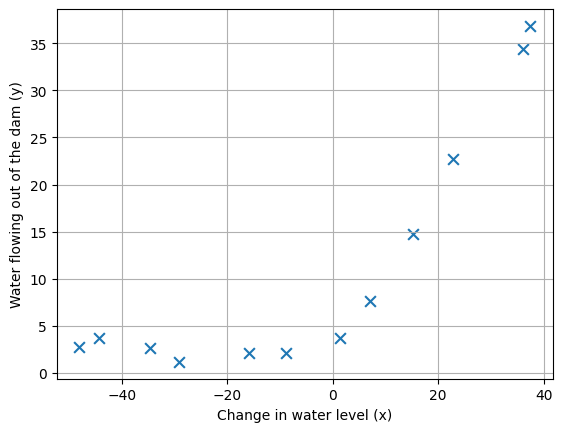
\includegraphics[width=1\textwidth]{./img/3.1.png}
            \caption{\label{fig:fig1}Diagramme de dispersion des données d'entraînement}  
        \end{center}
    \end{minipage}
\end{figure}

\begin{figure}[!h]
\begin{minted}[frame=lines, framesep=2mm, baselinestretch=1.2, fontsize=\footnotesize, linenos, breaklines=true]{python}
def plotData(X,y):
    pos = X[(y==1).flatten(),:]
    neg = X[(y==0).flatten(),:]
    plt.plot(pos[:,0], pos[:,1], '+', markersize=7, markeredgecolor='black', markeredgewidth=2) 
    plt.plot(neg[:,0], neg[:,1], 'o', markersize=7, markeredgecolor='black', markerfacecolor='yellow') 
    plt.legend(['Admitted (y=1)', 'Not admitted (y=0)'], loc='upper right', shadow=True, fontsize='x-large', numpoints=1) 
    plt.grid()
    plt.xlabel('Exam 1 score')
    plt.ylabel('Exam 2 score')
\end{minted}   
\captionof{listing}{Fonction plotData}
\end{figure}

    \subsection{Implémentation}

    Le modèle de régression linéaire est représenté par l'équation \ref{eq:regression_linear}. Cette équation nous permet d'obtenir une prédiction en fonction d'une entrée~$x$ et de $\theta$.
    
\begin{figure}[!h]
    \begin{minipage}{.48\linewidth}
\begin{minted}[frame=lines, framesep=2mm, baselinestretch=1.2, fontsize=\footnotesize, linenos, breaklines=true]{python}
def sigmoid(z):
        g = 1 / (1 + np.exp(-z))

    return  g
\end{minted}   
    \end{minipage}\hfill
    \begin{minipage}{.48\linewidth}
        \begin{align}\label{eq:regression_linear}
            h_\theta(x) = g (x^T \theta ) \\
            g(z)=\frac{1}{1-e^{-z}} 
        \end{align}
\end{minipage}
\end{figure}
    
    \noindent
    Pour que cette prédiction soit optimale, il est important de déterminer correctement les paramètres de notre modèle~: $\theta$. Pour cela, nous devons réaliser deux étapes~: Le calcul du coût $J(\theta)$ et une descente de gradient.

    \subsubsection{Calcul du coût $J(\theta)$}
    De la même manière que dans le TP1, le calcul du coût $J(\theta)$ permet de mesurer la qualité de la prédiction, si le coût est faible alors notre prédiction est proche des valeurs réelles et inversement si le coût est important. La formule utilisée pour calculer ce coût n'est pas la même pour une régression linéaire que pour une régression logistique. 
    
    \begin{equation}\label{eq:cout}
       J(\theta) = \frac{1}{m} \sum_{i=0}^{m-1}[-y^{(i)} log(h_\theta(x^{(i)})) - (1-y^{(i)}) log(1-h_\theta(x^{(i)}))]
    \end{equation}
 
    On remarque ici avec l'équation \ref{eq:cout} qui utilise l'équation \ref{eq:regression_linear}, que la seule valeur qui puisse influencer notre coût est $\theta$. Effectivement, les valeurs restantes : $x$, $y$ et $m$; sont les valeurs
    de notre problème qui sont déterminées et non modifiables.
    
    
    \vspace{.5cm}
    \noindent
    \textbf{Mise en application}
    \vspace{.2cm}

\begin{figure}[!h]
\begin{minted}[frame=lines, framesep=2mm, baselinestretch=1.2, fontsize=\footnotesize, linenos, breaklines=true]{python}
def costFunction(theta, X, y):
    # Initialize some useful values
    m,n = X.shape   
    theta = theta.reshape((n,1)) 
                
    predictions = sigmoid(X @ theta)
    J = (1/m) * np.sum(-y * np.log(predictions) - (1 - y) * np.log(1 - predictions))
    
    return  J

    """ return
    Cost at initial theta (zeros): 0.693147
    Expected cost (approx): 0.693
    """
\end{minted}   
\captionof{listing}{Fonction computeCost}
\end{figure}

\clearpage

\subsubsection{Descente de gradient}

La descente de gradient permet de minimiser le coût et donc d'obtenir les bonnes valeurs de theta pour réaliser une prédiction optimale.

\begin{equation}\label{eq:descente-gradient}
    \frac{\partial J(\theta)}{\partial \theta_j} = \frac{1}{m} \sum_{i=1}^{m} (h_\theta(x^{(i)}) - y^{(i)}) x_j^{(i)}
\end{equation}

\noindent
Cette formule pour calculer le gradient de la régression logistique comme pour le coût n'est pas identique à celle de la régression linéaire, en effet cela est dû aux définitions différentes de \( h_\theta (x) \).

\vspace{.5cm}
    \noindent
    \textbf{Mise en application}
    \vspace{.2cm}

\begin{figure}[!h]
\begin{minted}[frame=lines, framesep=2mm, baselinestretch=1.2, fontsize=\footnotesize, linenos, breaklines=true]{python}
def gradientFunction(theta, X, y):
    m = X.shape[0]  
    n = X.shape[1]   
    theta = theta.reshape((n,1)) 
    grad = 0
    for i in range(m):
        grad += (1/m) * (sigmoid(X[i] @ theta) - y[i]) * X[i]

    return grad

    """ return 
    theta: ['-25.1613', '0.2062', '0.2015']
    Expected theta (approx): -25.161 0.206 0.201
    
    -------------------------- 
    
    For a student with scores 45 and 85, we predict an admission probability of 0.776291
    Expected Proba (approx): 0.776
    
    -------------------------- 
    
    Train Accuracy: 89.000000
    Expected accuracy (approx): 89.0%
        """
\end{minted}   
\captionof{listing}{Fonction gradientFunction}
\end{figure}



\section{Régression linéaire avec plusieurs variables}
\subsection{Normalisation des caractéristiques}

Dans ce problèmes nous avons des caractéristiques qui ont des échelles radicallement différentes \textit{(exemple 2100 sq-ft pour 3 chambres)}. Il est intéressant de normaliser c'est données pour les ramener à une échelle comune, 
ce qui permet d'interpréter plus facilement les résultat et rendre les calculs plus stable et rapide. Grâce à la normalisation on peut être sûr que chaque caractéristiques contribue équitablement à la prédiction du modèle, indépendamment de son échelle initiale. \\

\noindent
Pour réaliser la normalisation nous pouvons établire les formules suivantes:

\begin{figure}[!h]
    \centering
    \begin{minipage}{.33\linewidth}
        \begin{equation*}
            X_{norm} = \frac{X - \mu}{\sigma}
        \end{equation*}
    \end{minipage}\hfill\vline
    \begin{minipage}{.33\linewidth}
        \begin{equation*}
            \mu = \frac{1}{m} \sum_{i=0}^{m-1}x_j^{(i)}
        \end{equation*}        
    \end{minipage}\hfill\vline
    \begin{minipage}{.33\linewidth}
        \begin{equation*}
            \sigma = \sqrt{\frac{1}{m} \sum_{i=1}^{m} \left(x_j^{(i)} - \mu\right)^2}
        \end{equation*}                
    \end{minipage}
\end{figure}

\begin{itemize}
    \item $\mu$ La moyenne de chaques caractéristiques
    \item $\sigma$ L'écart type de chaques caractéristiques
    \item $X_{norm}$ Caractéristiques normalisées
    \item $x_j^{(i)}$ La caractéristique de la ligne $j$ à la colonne $i$
\end{itemize}

\clearpage

\vspace{.5cm}
\noindent
\textbf{Mise en application}
\vspace{.2cm}


\begin{figure}[!h]
    \begin{minipage}{.48\linewidth}
\begin{minted}[frame=lines, framesep=2mm, baselinestretch=1.2, fontsize=\footnotesize, linenos, breaklines=true]{python}
def featureNormalize(X):
    mu = np.mean(X, axis=0)
    sigma = np.std(X, axis=0)
    X_norm = (X - mu) / sigma

    return X_norm, mu, sigma
\end{minted}   
\captionof{listing}{Fonction featureNormalize}
    \end{minipage}\hfill
    \begin{minipage}{.48\linewidth}
        \begin{equation*}
            \begin{aligned}
                \mu &= [2000.68085106 \quad 3.17021277] \\
                \sigma &= [7.86202619e+02 \quad 7.52842809e-01]
            \end{aligned}
        \end{equation*}  
    \end{minipage}
\end{figure}


\subsection{Descente de gradient}

La descente de gradient de ce second problème, suit la même méthodologie. La seule différence est qu'ici on à plusieurs caractéristiques. \\
Nos fonction précédentes sont adapté pour un calcul de coût et une descente de gradient à plusieurs caractéristiques, nous pouvons réutiliser les mêmes fonctions.

\begin{figure}[!h]
\begin{minted}[frame=lines, framesep=2mm, baselinestretch=1.2, fontsize=\footnotesize, linenos, breaklines=true]{python}
def computeCostMulti(X, y, theta):  
   m = y.size
   J = 0

   for i in range(0, m):
      J += (1/(2*m)) * (X[i].T @ theta - y[i])**2
   
   return J
\end{minted}   
\captionof{listing}{Fonction computeCostMulti}\label{listing:computeCostMulti}
\end{figure}


\begin{figure}[!h]
\begin{minted}[frame=lines, framesep=2mm, baselinestretch=1.2, fontsize=\footnotesize, linenos, breaklines=true]{python}
def gradientDescentMulti(X, y, theta, alpha, num_iters):  
    m = y.size  # number of training examples
    n = theta.size # number of parameters
    cost_history = np.zeros(num_iters)
    theta_history = np.zeros((n,num_iters))

    for n_iter in range(num_iters):
        for j in range(n):
            res = 0
            for i in range(m):
                res += (X[i].T @ theta - y[i]) * X[i][j]
            
            theta[j] = theta[j] - alpha * (1/m) * res

        cost_history[n_iter] = computeCostMulti(X, y, theta)
        theta_history[:,n_iter] = theta.reshape((n,))
              
    return theta, cost_history, theta_history
\end{minted}   
\captionof{listing}{Fonction gradientDescentMulti}\label{listing:gradientDescentMulti}
\end{figure}


Suite à notre descente de gradient, on constate sur la figure \ref{fig:fig4} que le coût $J(\theta)$ converge vers un minimum. On peut donc considérer que nos valeurs de $\theta$ sont optimal pour réaliser une prédiction proche de la réalité.

\begin{figure}[!h]
    \begin{minipage}{.48\linewidth}
        \begin{center}
            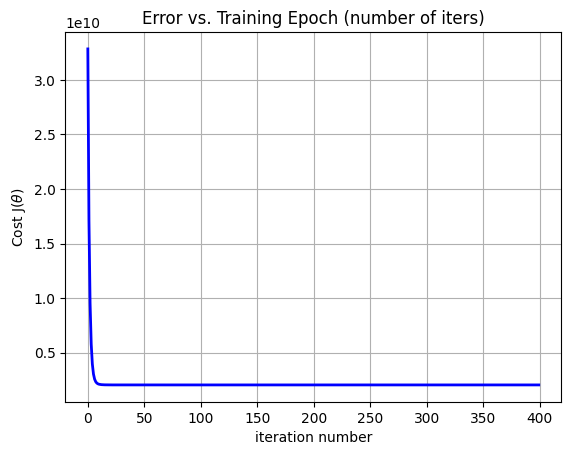
\includegraphics[width=1\textwidth]{./img/5-2.png}
            \caption{\label{fig:fig4}Convergence de $J(\theta)$ en fonction des itérations avec $\alpha = 0.3$}  
        \end{center}
    \end{minipage}\hfill
    \begin{minipage}{.48\linewidth}
        \begin{equation*}
            \begin{aligned}
                \theta_0 &= 340412.65957447 \\
                \theta_1 &= 109447.79 \\
                \theta_2 &= -6578.35
            \end{aligned}
        \end{equation*}  

        Prédiction pour une maison de 1650 \textit{sq-ft} et 3 chambres de 293081.46\$
    \end{minipage}
\end{figure}

\subsubsection{Sélection du taux d'apprentissage}

Comme expliqué précédement il est important de séléctionner correctement le taux d'apprentissage, si celui-ci est trop important alors la descente de gradient peut divergé d'un minimum, si il est trop petit alors le processus peut échouer dû à des 
valeurs trop importantes.

\vspace{.5cm}
\noindent
\textbf{Trop petit, $\alpha = 0.001$}
\vspace{.2cm}

\begin{figure}[!h]
    \begin{minipage}{.48\linewidth}
        \begin{center}
            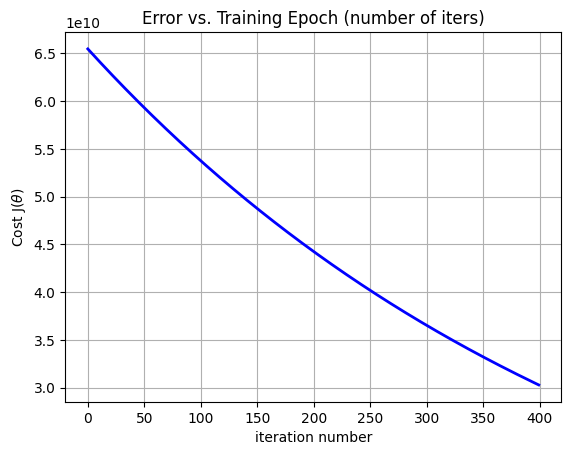
\includegraphics[width=1\textwidth]{./img/lowlearningrateng.png}
            \caption{\label{fig:fig5}Convergence de $J(\theta)$ en fonction des itérations avec $\alpha = 0.001$}  
        \end{center}
    \end{minipage}\hfill
    \begin{minipage}{.48\linewidth}
        \begin{equation*}
            \begin{aligned}
                \theta_0 &= 112272.89 \\
                \theta_1 &= 33255.72 \\
                \theta_2 &= 14509.19
            \end{aligned}
        \end{equation*}  

        Prédiction pour une maison de 1650 \textit{sq-ft} et 3 chambres de $94158.94$\$
    \end{minipage}
\end{figure}


Dans ce cas le taux d'apprentissage choisis est trop faible, on le constate grâce à l'allure de la courbe mais également avec les résultats obtenus. Un résultat cohérent se rapproche de l'allure de la figure \ref{fig:fig4}.

\subsection{Exercice facultatif: Equations normales}

La régression linéaire par équations normales donne un résultat similaire à la descente de gradient, mais ce n'est pas un algorithme itératif. L'équation \ref{eq:eq_normal} nous permet d'obtenir directement une 
valeur optimal de $\theta$.

\begin{equation}\label{eq:eq_normal}
    \theta = (X^T X)^{-1} X^T y
\end{equation}  


\vspace{.5cm}
\noindent
\textbf{Mise en application}
\vspace{.2cm}


\begin{figure}[!h]
    \begin{minipage}{.48\linewidth}
\begin{minted}[frame=lines, framesep=2mm, baselinestretch=1.2, fontsize=\footnotesize, linenos, breaklines=true]{python}
def normalEqn(X,y):
    theta = np.linalg.inv((X.T @ X)) @ X.T @ y

    return theta
\end{minted}   
\captionof{listing}{Fonction normalEqn}\label{listing:normalEqn}
    \end{minipage}\hfill
    \begin{minipage}{.48\linewidth}
        Prédiction pour une maison de 1650 \textit{sq-ft} et 3 chambres de $293081.46$\$ avec la méthode des équations normal. \\
        Le résultat est similaire de celui obtenus par la méthode de la descente de gradient avec une valeur de $\alpha = 0.3$.
    \end{minipage}
\end{figure}

\section{Questions}

\begin{enumerate}
    \item \textbf{Définissez les termes:}
    \begin{itemize}
        \item \textbf{Approches supervisées} \\
        L'approche supervisée est utilisée quand on a un certains nombres de données connus et correctes. C'est données sont utilisées pour entrainer le modèle pour que celui-ci puisse nous 
        donner une prévision proche de la réalité. Nous avons donc appliqué une approche supervisée dans ce TP.

        \item \textbf{Approches non supervisées} \\
        Il s'agit de l'inverse de l'approche supervisée, ici on lui demande un résultat à l'aide de données aléatoires.

        \item \textbf{Régression} \\
        Utilisé pour déterminer une prédiction optimale à l'aide d'une relation linéaire entre une variable dépendante et plusieurs variables indépendantes.

        \item \textbf{Classification} \\
        Utilisé pour déterminer à qu'elle classe appartient une observation à partir de précédentes connus.

    \end{itemize}
    \item \textbf{Représenter en un schéma général, les processus d'apprentissage et de prédiction ?} \\
    \begin{figure}[!h]
        \begin{center}
            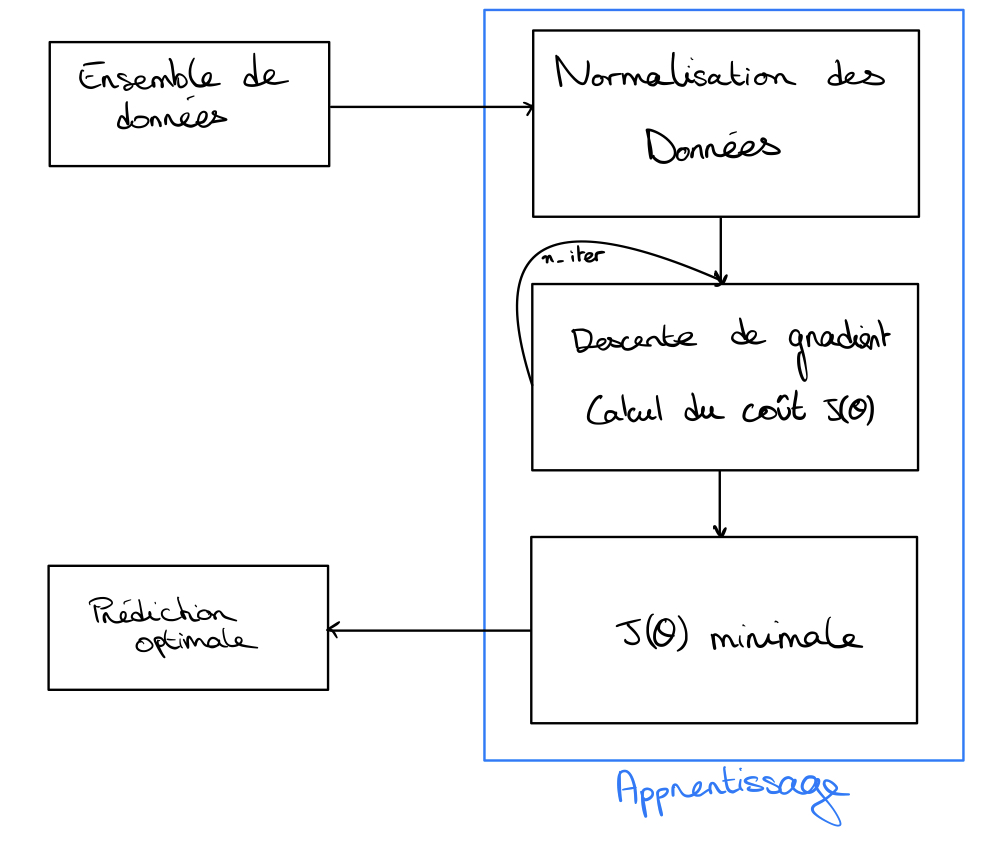
\includegraphics[width=.38\textwidth]{./img/schema.jpeg}
            \caption{\label{fig:fig6}Schéma général d'apprentissage}  
        \end{center}
    \end{figure}
    \item \textbf{Comment fonctionne l'apprentissage ? Par quels moyens ? A quoi sert la fonction de coût ? Comment est-résolu le problème ? Connaissez vous d'autres moyens de le résoudre ?} \\
    La méthode d'apprentissage par régression linéaire fonctionne grâce à l'ajustement du paramètre de notre modèle $\theta$. Pour ce faire, il faut minimiser la fonction de coût \textit{(erreur entre la prédiction et la réalité)} à l'aide
    d'une descente de gradient ce qui permet d'obtenir un $\theta$ pour réaliser une prédiction optimale. \\
    On peut résoudre ce problème avec une descente de gradient, mais également avec les équations normales.

    \item \textbf{Pourquoi faut-il parfois normaliser les descripteurs (features) ?} \\
    Il est intéressant de normaliser les données pour les ramener à une échelle commune, 
    ce qui permet d'interpréter plus facilement les résultats et rendre les calculs plus stables et rapides. Grâce à la normalisation, on peut être sûr que chaque caractéristique contribuent équitablement à la prédiction du modèle, indépendamment de son échelle initiale. \\
    
\end{enumerate}


\end{document}